\documentclass[handout]{beamer}
\usepackage{pgfpages}
\pgfpagesuselayout{4 on 1}[border shrink=5mm]
\usetheme{Madrid}

\usepackage[utf8]{inputenc}
\usepackage{graphicx}
\graphicspath{ {Image/} }

\title{Réseau PERT et Diagramme de Gantt}

\subtitle{Ou comment gérer le déroulement d'un projet}

\author{S.Juhel \and C.Barcelo}

\institute[UM2]
{
  Département informatique
  Université de Montpellier 2
}

\date{TCCP, 2014}

\subject{Réseau PERT et Diagramme de Gantt}
% Uniquement dans le PDF

\pgfdeclareimage[height=0.5cm]{university-logo}{Image/logo.png}
\logo{\pgfuseimage{university-logo}}

\AtBeginSubsection[]
{
  \begin{frame}<beamer>{Sommaire}
    \tableofcontents[currentsection,currentsubsection]
  \end{frame}
}

% Début du document
\begin{document}

\begin{frame}
  \titlepage
\end{frame}

\begin{frame}{Sommaire}
  \tableofcontents
\end{frame}

\section{Introduction}

\begin{frame}{Introduction}{Gestion du temps pour un projet}
    \begin{block}{Constat}
        La gestion du temps pour un projet est une problématique courante
    \end{block}
    \pause
    \begin{block}{Contrainte}
        La collaboration requiert une solution qui soit claire pour l'ensemble des participants
    \end{block}
    \pause
    \begin{block}{Solution}
        Utilisation d'outils spécifiques représentant graphiquement l'avancement du projet.
    \end{block}
\end{frame}

\begin{frame}{Introduction}
    Deux outils complémentaires existent :
    \begin{itemize}
    \item {Diagramme de Gantt (d'après Henry L. Gantt 1910)}
    \item {Réseau PERT (\textit{Program Evaluation and Review Technology} 1958)}
    \end{itemize}
\end{frame}


\section{Diagramme de Gantt}
    
\subsection{Qu'est-ce-qu'un diagramme de Gantt ?}

\begin{frame}{Objectifs du diagramme de Gantt}
    Un diagramme de Gantt répond à deux objectifs :
    \pause
    \begin{block}{Planification}
        Définir les dates clefs du projet
    \end{block}
    \pause
    \begin{block}{Communication}
        Permettre aux participants de connaître le déroulement global du projet
    \end{block}
\end{frame}

\begin{frame}{Informations fournies par le diagramme}
  Un diagramme de Gantt permet de visualiser :
  \begin{itemize}
  \item {Les différentes tâches à envisager}
  \item {Les dates de réalisation d'un projet}
  \item {Les marges existantes pour chaque tâche}
  \item {Les éventuels retards du projet}
  \item {Le chevauchement éventuel des tâches}
  \end{itemize}
\end{frame}


\subsection{Construction d'un diagramme de Gantt}

\begin{frame}{Construction d'un diagramme de Gantt}
    Composition minimal d'un diagramme :
    \begin{itemize}
    \item {Un axe temporel en abscisse}
    \item {L'ensemble des tâches en ordonnée}
    \end{itemize}
     On représente le temps estimé pour chaque tâche avec une barre horizontale. \newline{}
    Les extrémités de la barre modélisent le début et la fin prévues pour la tâche.
\end{frame}

\begin{frame}{Informations complémentaire}
    Il est possible de completer le diagramme avec d'autres informations
	\begin{itemize}
		\item {Les ressources humaines}
		\item {Les ressources matérielles }
		\item {Une visualisation de la date actuelle (sur logiciel)}
	\end{itemize}
\end{frame}

\subsection{Exemple de diagramme}
\begin{frame}{Exemple de diagramme}
    \begin{figure}
    \centering
    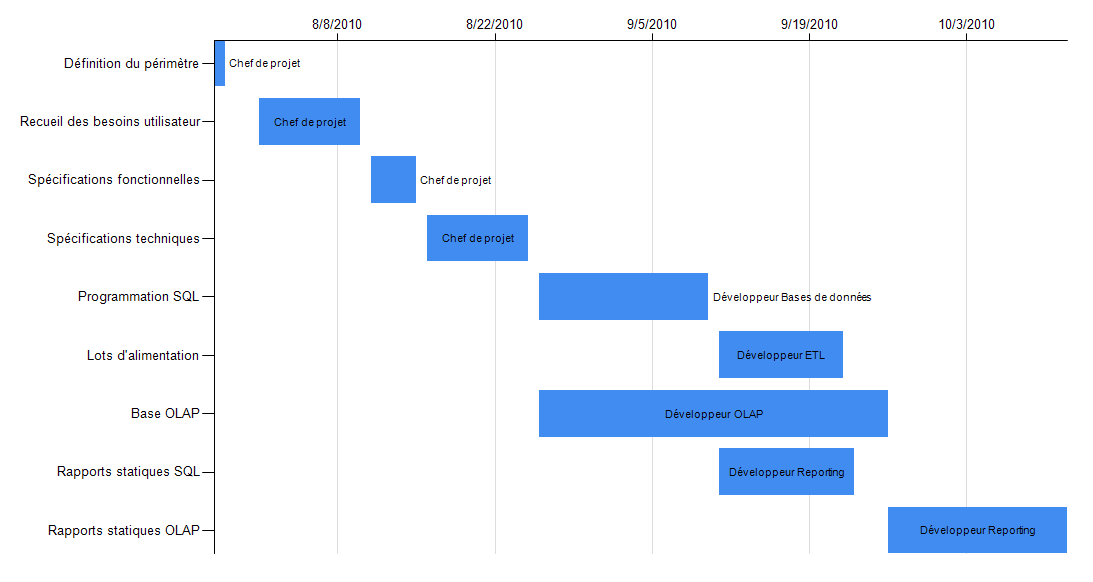
\includegraphics[scale=0.40]{gantt.png}
    \caption{Un exemple simple de diagramme de Gantt}
    \label{fig:Gantt1}
    \end{figure}
\end{frame}


\begin{frame}{Exemple de diagramme}
    \begin{figure}
    \centering
    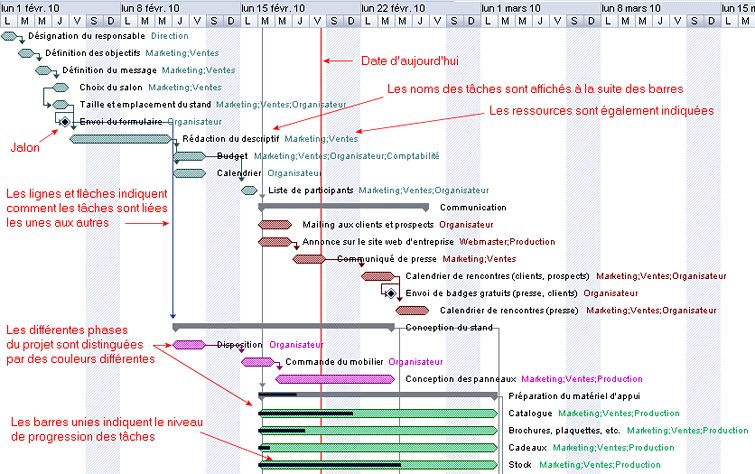
\includegraphics[scale=0.35]{gantt2.png}
    \caption{Un exemple moins simple de diagramme de Gantt}
    \label{fig:Gantt2}
    \end{figure}
\end{frame}

\subsection{Limites du diagramme de Gant}

\begin{frame}{Les inconvénients}
    Il existe des limites au diagramme de Gantt :
    \vspace{\baselineskip}
    \begin{itemize}
    \item{Tâches en concurrence sur l'utilisation des ressources}
    \item{Peut devenir très complexe pour les projets très importants}
    \item{Doit être constamment tenu à jour}
    \item{La taille de la barre n’indique pas forcément la quantité de travail.}
    \end{itemize}
\end{frame}

\section{Réseau PERT}

\subsection{Qu'est-ce-que le réseau PERT ?}

\begin{frame}{Objectifs d'un Réseau PERT}
    Un réseau PERT répond à deux objectifs :
    \pause
    \begin{block}{Analyse}
        Analyser une suite de tâche dans un projet
    \end{block}
    \pause
    \begin{block}{Représentation}
        Représenter cette suite de tâche de façon logique
    \end{block}
    \vspace{\baselineskip}
    \pause
    Un réseau PERT vient souvent compléter ou préciser un diagramme de Gantt
\end{frame}

\subsection{Réalisation}

\begin{frame}{Réalisation}
    Pour concevoir un Réseau PERT il faut :
    \begin{itemize}
     \item {
    Structurer le projet
    \pause % The slide will pause after showing the first item
  }
  \item {   
    Analyser et évaluer les tâches
    \pause
  }
  \item {   
    Schématiser le réseau de tâches
      }
\end{itemize}
\end{frame}

\subsection{Informations données par le réseau}

\begin{frame}{Contenu du réseau}
    Le réseau de PERT se compose des différentes tâches du projet présentées de         manière ordonnée.\\
    \pause
    \vspace{\baselineskip}
    Pour chacune des tâches on donne :
    \begin{itemize}
        \item {   
        un identifiant(sa position dans la réalisation des tâches)
        }
        \item{
        sa date au plus tôt
        }
        \item{
        sa date au plus tard
        }


  \end{itemize}
\end{frame}

\subsection{Exemple de réseau}
\begin{frame}{Exemple de réseau}
    \begin{figure}
    \centering
    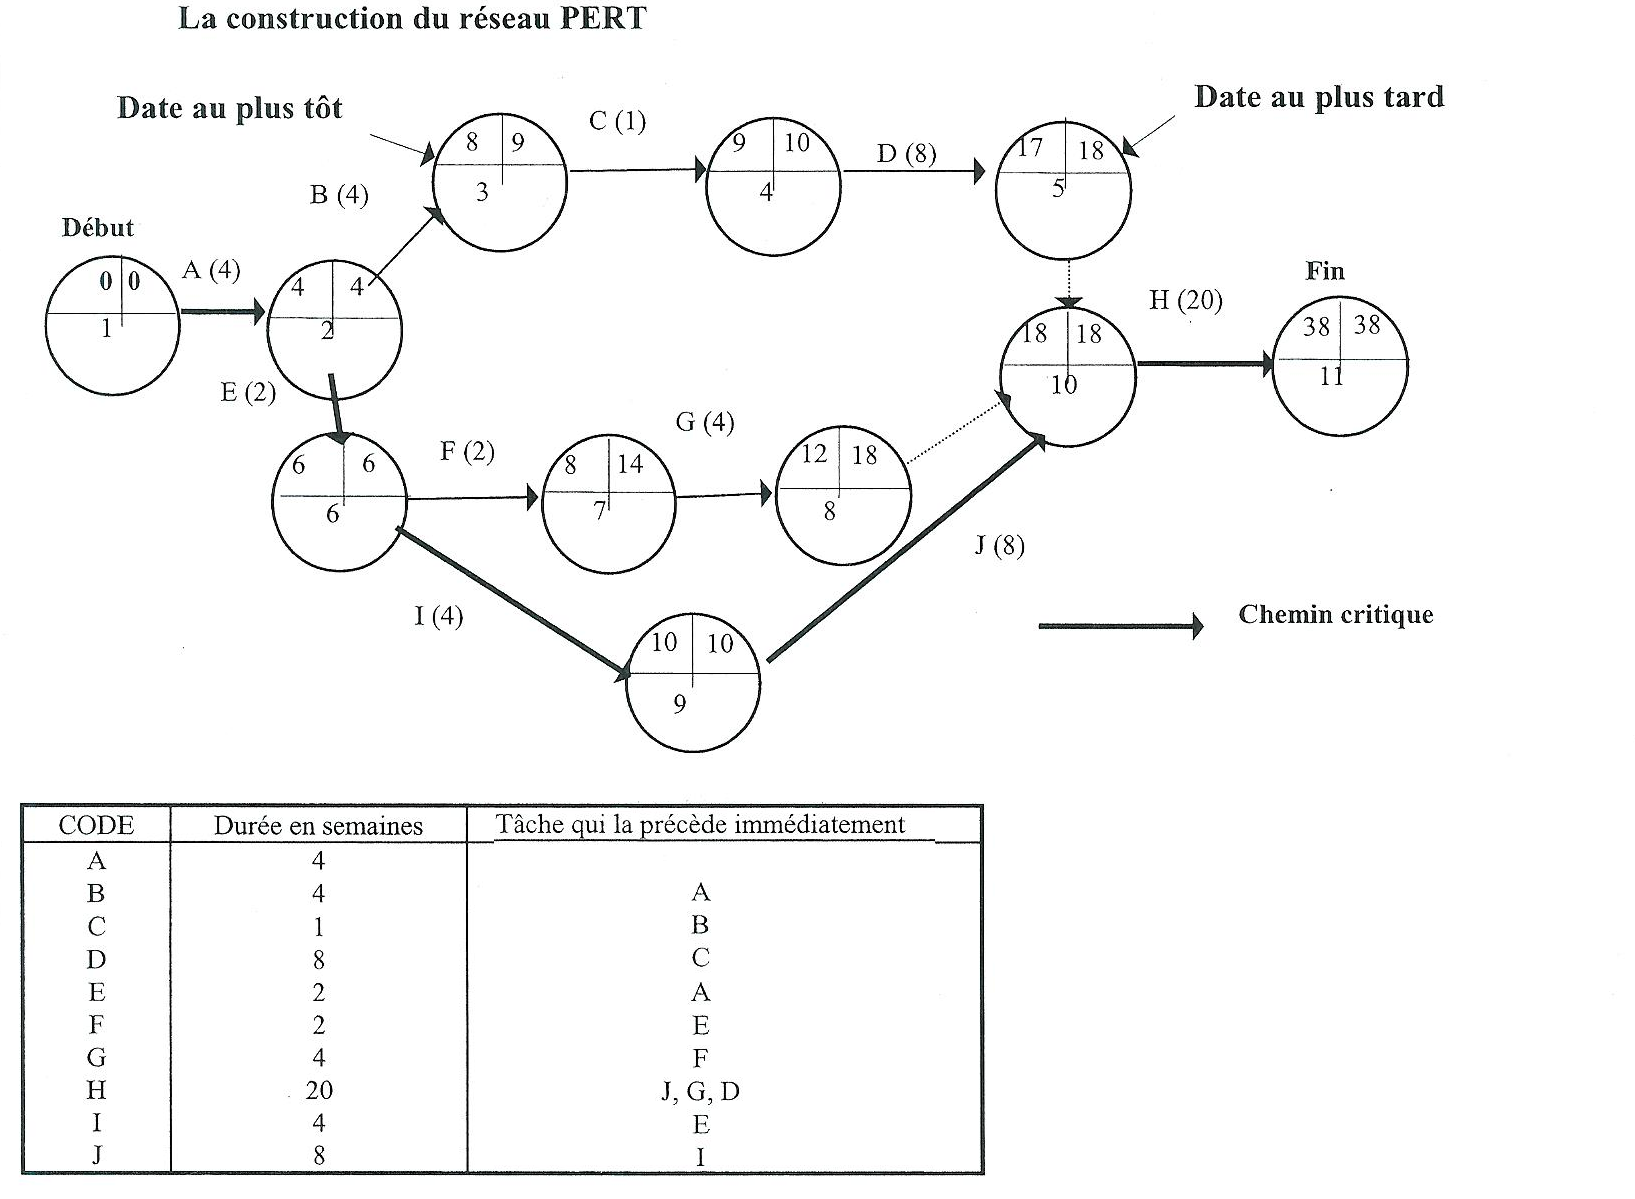
\includegraphics[scale=0.20]{pert.png}
    \caption{Exemple de Réseau PERT}
    \label{fig:PERT}
    \end{figure}
\end{frame}

\section{Les outils informatiques}
\subsection*{Les outils informatiques}
\begin{frame}{Les outils informatiques}
    \begin{itemize}
    \item GanttProject (Dernière version : 2014) : Libre, Java, Multiplate-forme
    \item Open Workbench (Dernière version : 2006) : Gratuit, Java, Uniquement sur Windows
    \item Microsoft Project (Dernière version : 2013) : Propriétaire, C++, Uniquement sur Windows, le plus utilisé dans le monde
    \item ProjectLibre (Dernière version : 2014) : Libre, Java, Multiplate-forme, s'inspire de Microsoft Project
    \item Et plein d'autre (Genius Project, Open Project, etc...)
    \end{itemize}
    \vspace{\baselineskip}
    Il existe aussi des paquets pour \LaTeX{} permettant d'intégrer des diagrammes de Gantt/PERT.
\end{frame}

\section{Conclusion}
\subsection*{Conclusion}
\begin{frame}{Conclusion}
    \begin{itemize}
    \item{La gestion du temps pour un projet est un élément très important}
    \item{Diagramme de Gantt et d'un réseau PERT apportent une solution efficace}
    \item{Utile dans la relation client}
    \item{La mise en place est d'autant plus complexe que le projet est important}
    \end{itemize}
\end{frame}

\begin{frame}{}
    \centering
    \textbf{Merci de votre attention}
\end{frame}

\end{document}


